\documentclass[12pt,twoside]{article}
%%%%%%%%%%%%%%%%%%%%%%%%%%%%%%%%%%%%%%%%%%%%%%%%%%%%%%%%%%%%%
% Meta informations:
\newcommand{\trauthor}{Sayantan Auddy}
\newcommand{\trtype}{Seminar Paper} %{Seminararbeit} %{Proseminararbeit}
\newcommand{\trcourse}{Independent Study}
\newcommand{\trtitle}{Biped Locomotion using Central Pattern Generators}
\newcommand{\trmatrikelnummer}{6640595}
\newcommand{\tremail}{4auddy@informatik.uni-hamburg.de}
\newcommand{\trarbeitsbereich}{Knowledge Technology, WTM}
\newcommand{\trdate}{03.11.2016}

%%%%%%%%%%%%%%%%%%%%%%%%%%%%%%%%%%%%%%%%%%%%%%%%%%%%%%%%%%%%%
% Languages:

% Falls die Ausarbeitung in Deutsch erfolgt:
% \usepackage[german]{babel}
% \usepackage[T1]{fontenc}
% \usepackage[latin1]{inputenc}
% \usepackage[latin9]{inputenc}	 				
% \selectlanguage{german}

% If the thesis is written in English:
\usepackage[english]{babel} 						
\selectlanguage{english}

%%%%%%%%%%%%%%%%%%%%%%%%%%%%%%%%%%%%%%%%%%%%%%%%%%%%%%%%%%%%%
% Bind packages:
\usepackage{acronym}                    % Acronyms
\usepackage{algorithmic}				% Algorithms and Pseudocode
\usepackage{algorithm}					% Algorithms and Pseudocode
\usepackage{amsfonts}                   % AMS Math Packet (Fonts)
\usepackage{amsmath}                    % AMS Math Packet
\usepackage{amssymb}                    % Additional mathematical symbols
\usepackage{amsthm}
\usepackage{booktabs}                   % Nicer tables
%\usepackage[font=small,labelfont=bf]{caption} % Numbered captions for figures

\usepackage{color}                      % Enables defining of colors via \definecolor
\definecolor{uhhRed}{RGB}{254,0,0}      % Official Uni Hamburg Red
\definecolor{uhhGrey}{RGB}{122,122,120} % Official Uni Hamburg Grey
\usepackage{fancybox}                   % Gleichungen einrahmen
\usepackage{fancyhdr}					% Packet for nicer headers
%\usepackage{fancyheadings}             % Nicer numbering of headlines

%\usepackage[outer=3.35cm]{geometry} 	% Type area (size, margins...) !!!Release version
%\usepackage[outer=2.5cm]{geometry} 	% Type area (size, margins...) !!!Print version
%\usepackage{geometry} 					% Type area (size, margins...) !!!Proofread version
\usepackage[outer=3.15cm]{geometry} 	% Type area (size, margins...) !!!Draft version
\geometry{a4paper,body={5.8in,9in}}

\usepackage{graphicx}                   % Inclusion of graphics
%\usepackage{latexsym}                  % Special symbols
\usepackage{longtable}					% Allow tables over several pages
\usepackage{listings}                   % Nicer source code listings
\usepackage{multicol}					% Content of a table over several columns
\usepackage{multirow}					% Content of a table over several rows
\usepackage{rotating}					% Alows to rotate text and objects
\usepackage[hang]{subfigure}            % Allows to use multiple (partial) figures in a fig
%\usepackage[font=footnotesize,labelfont=rm]{subfig}	% Pictures in a floating environment
\usepackage{tabularx}					% Tables with fixed width but variable rows
\usepackage{url,xspace,boxedminipage}   % Accurate display of URLs
\usepackage{multirow}
\usepackage{tabulary}

%%%%%%%%%%%%%%%%%%%%%%%%%%%%%%%%%%%%%%%%%%%%%%%%%%%%%%%%%%%%%
% Configurationen:

\hyphenation{whe-ther} 					% Manually use: "\-" in a word: Staats\-ver\-trag

%\lstloadlanguages{C}                   % Set the default language for listings
\DeclareGraphicsExtensions{.pdf,.svg,.jpg,.png,.eps} % first try pdf, then eps, png and jpg
\graphicspath{{./src/}} 				% Path to a folder where all pictures are located
\pagestyle{fancy} 						% Use nicer header and footer

% Redefine the environments for floating objects:
\setcounter{topnumber}{3}
\setcounter{bottomnumber}{2}
\setcounter{totalnumber}{4}
\renewcommand{\topfraction}{0.9} 		%Standard: 0.7
\renewcommand{\bottomfraction}{0.5}		%Standard: 0.3
\renewcommand{\textfraction}{0.1}		%Standard: 0.2
\renewcommand{\floatpagefraction}{0.8} 	%Standard: 0.5

% Tables with a nicer padding:
\renewcommand{\arraystretch}{1.2}

%%%%%%%%%%%%%%%%%%%%%%%%%%%%
% Additional 'theorem' and 'definition' blocks:
\theoremstyle{plain}
\newtheorem{theorem}{Theorem}[section]
%\newtheorem{theorem}{Satz}[section]	% Wenn in Deutsch geschrieben wird.
\newtheorem{axiom}{Axiom}[section] 	
%\newtheorem{axiom}{Fakt}[chapter]		% Wenn in Deutsch geschrieben wird.
%Usage:%\begin{axiom}[optional description]%Main part%\end{fakt}

\theoremstyle{definition}
\newtheorem{definition}{Definition}[section]

%Additional types of axioms:
\newtheorem{lemma}[axiom]{Lemma}
\newtheorem{observation}[axiom]{Observation}

%Additional types of definitions:
\theoremstyle{remark}
%\newtheorem{remark}[definition]{Bemerkung} % Wenn in Deutsch geschrieben wird.
\newtheorem{remark}[definition]{Remark} 

%%%%%%%%%%%%%%%%%%%%%%%%%%%%
% Provides TODOs within the margin:
\newcommand{\TODO}[1]{\marginpar{\emph{\small{{\bf TODO: } #1}}}}

%%%%%%%%%%%%%%%%%%%%%%%%%%%%
% Abbreviations and mathematical symbols
\newcommand{\modd}{\text{ mod }}
\newcommand{\RS}{\mathbb{R}}
\newcommand{\NS}{\mathbb{N}}
\newcommand{\ZS}{\mathbb{Z}}
\newcommand{\dnormal}{\mathit{N}}
\newcommand{\duniform}{\mathit{U}}

\newcommand{\erdos}{Erd\H{o}s}
\newcommand{\renyi}{-R\'{e}nyi}
%%%%%%%%%%%%%%%%%%%%%%%%%%%%%%%%%%%%%%%%%%%%%%%%%%%%%%%%%%%%%
% Document:
\begin{document}
\renewcommand{\headheight}{14.5pt}

\fancyhead{}
\fancyhead[LE]{ \slshape \trauthor}
\fancyhead[LO]{}
\fancyhead[RE]{}
\fancyhead[RO]{ \slshape \trtitle}

%%%%%%%%%%%%%%%%%%%%%%%%%%%%
% Cover Header:
\begin{titlepage}
	\begin{flushleft}
		Universit\"at Hamburg\\
		Department Informatik\\
		\trarbeitsbereich\\
	\end{flushleft}
	\vspace{3.5cm}
	\begin{center}
		\huge \trtitle\\
	\end{center}
	\vspace{3.5cm}
	\begin{center}
		\normalsize\trtype\\
		[0.2cm]
		\Large\trcourse\\
		[1.5cm]
		\Large \trauthor\\
		[0.2cm]
		\normalsize Matr.Nr. \trmatrikelnummer\\
		[0.2cm]
		\normalsize\tremail\\
		[1.5cm]
		\Large \trdate
	\end{center}
	\vfill
\end{titlepage}

	%backsite of cover sheet is empty!
\thispagestyle{empty}
\hspace{1cm}
\newpage

%%%%%%%%%%%%%%%%%%%%%%%%%%%%
% Abstract:

% Abstract gives a brief summary of the main points of a paper:
\section*{Abstract}
  

% Lists:
\setcounter{tocdepth}{2} 					% depth of the table of contents (for Seminars 2 is recommented)
\tableofcontents
\pagenumbering{arabic}
\clearpage

%%%%%%%%%%%%%%%%%%%%%%%%%%%%
% Content:

% the actual content, usually separated over a number of sections
% each section is assigned a label, in order to be able to put a
% crossreference to it

\graphicspath{{images/}}

\section{Introduction}
\label{sec:introduction}


\section{Section 2}

\subsection{Section 2.1}

\section{Properties of the Matsuoka oscillator}

\subsection{Using proprioceptive feedback to control the mean position}
On its own, the Matsuoka oscillator produces oscillations about an arbitrary position, and the system itself is dynamically unstable. However, with the introduction of a feedback term, the mean position of oscillations can be controlled \cite{ronsse2009computational}. This is shown in figure \ref{fig:change-avg-pos}.

\begin{figure}[htbp]
\centering     %%% not \center
\subfigure[Torque output of the oscillator]{\label{fig:b}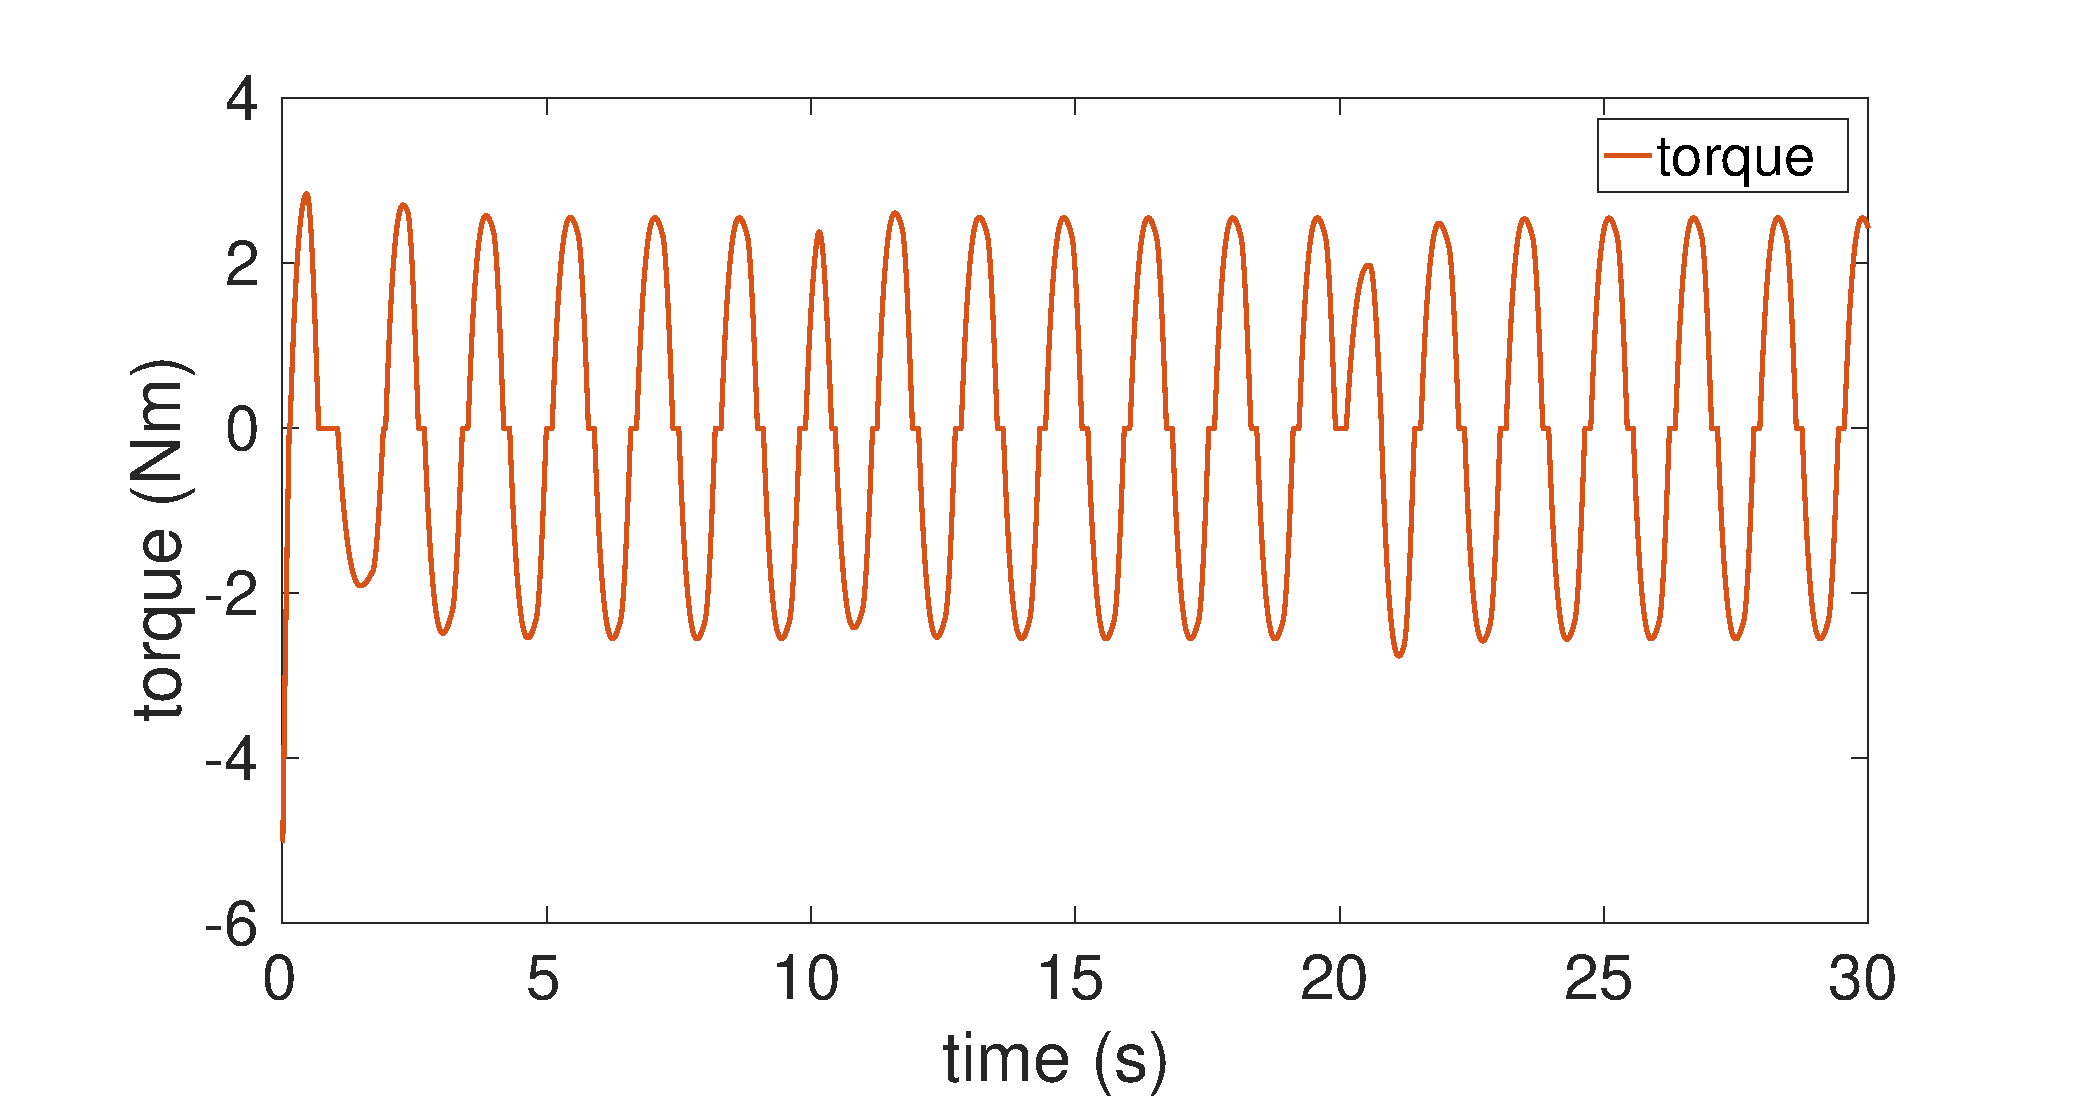
\includegraphics[scale=0.33]{figures/1-2-torque-for-change-average-position.eps}}
\subfigure[Joint position and average joint position]{\label{fig:a}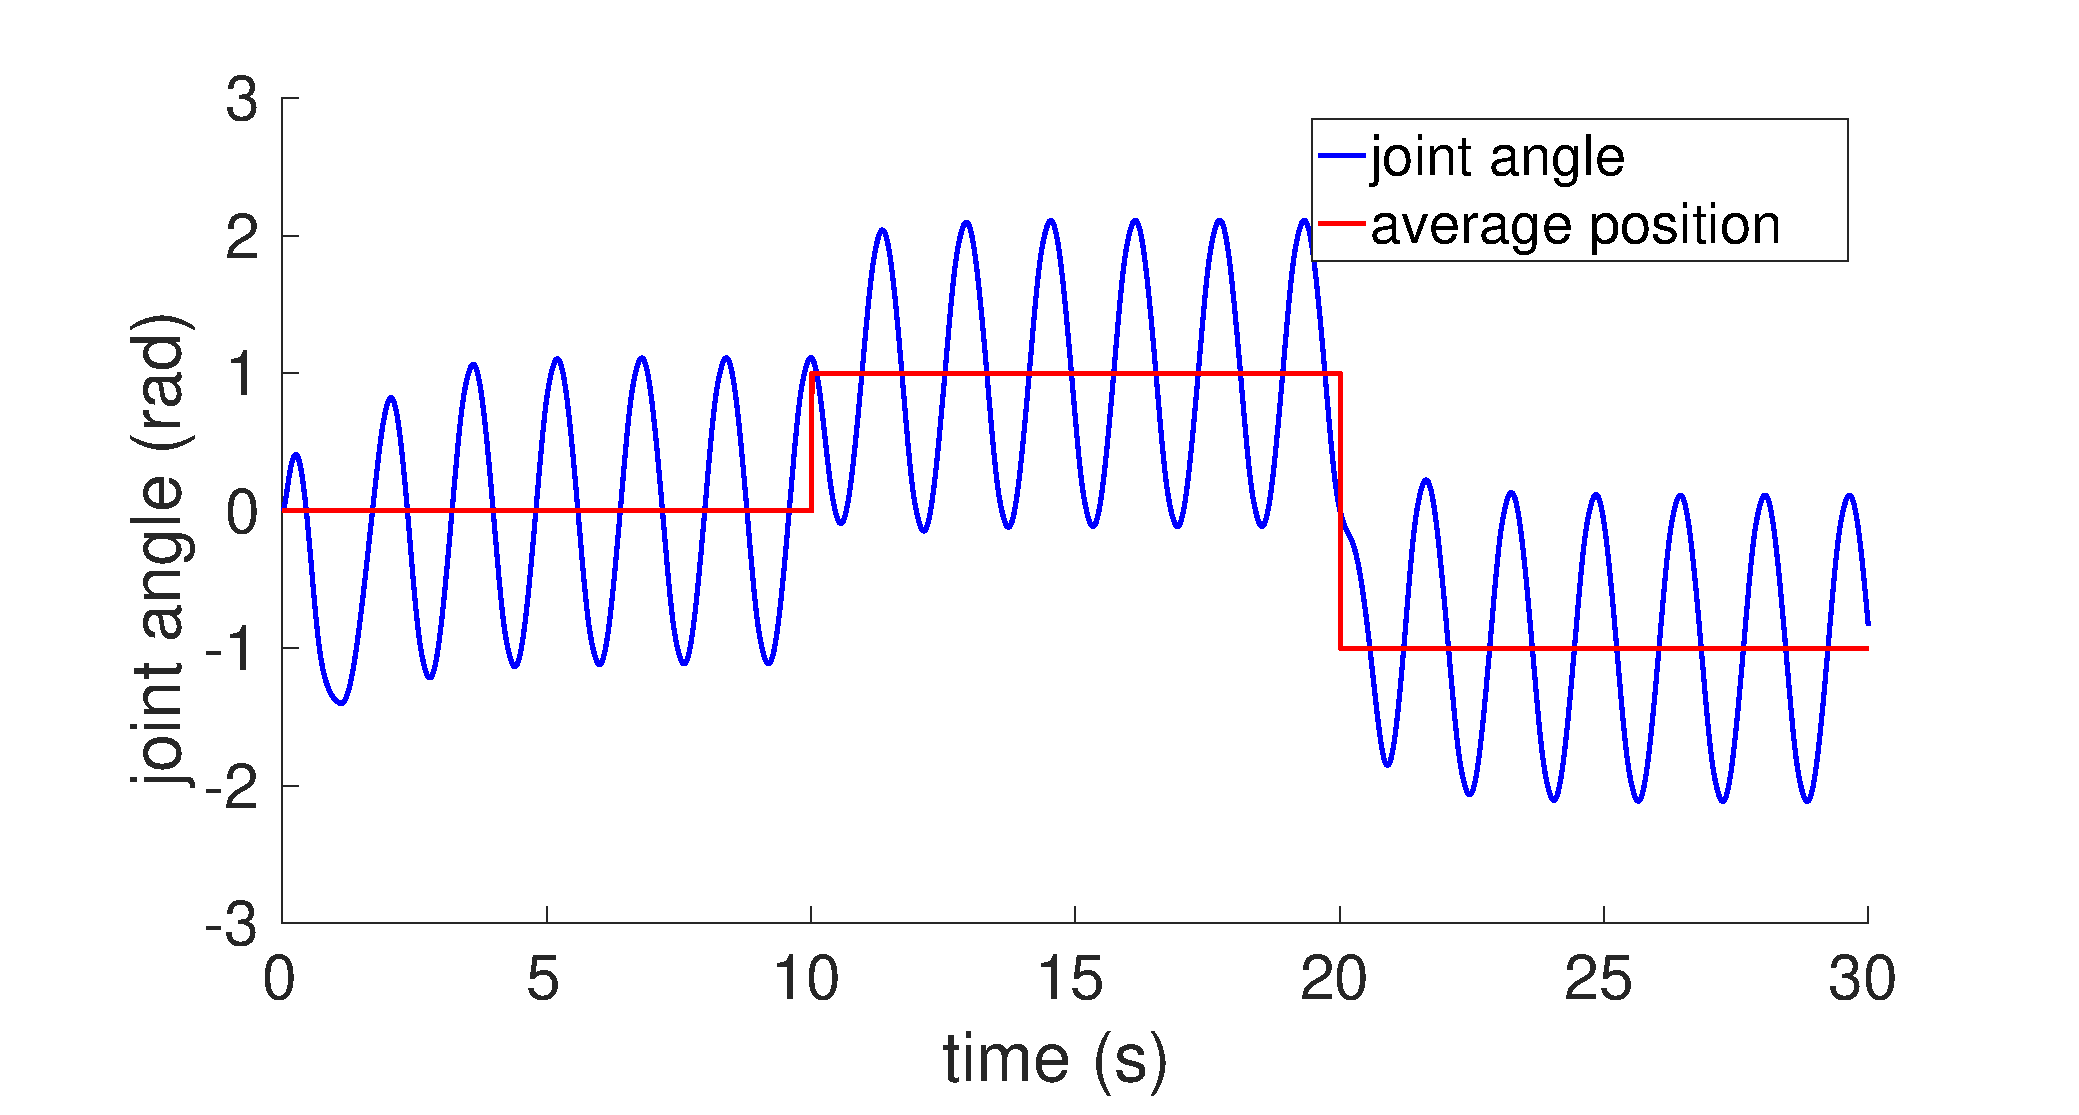
\includegraphics[scale=0.33]{figures/1-1-change-average-position.eps}}
\caption{Changing the average position of oscillation}
\label{fig:change-avg-pos}
\end{figure}

\subsection{Controlling the amplitude of the joint angle oscillations}
The tonic input to the oscillator is linearly related to the amplitude of the torque output and also approximately linearly to the amplitude of the position oscillations. Here the tonic input was linearly increased from 1.0 to 4.0 over 30 seconds, and as shown in figure \ref{fig:change-amp}, the amplitude of both the oscillations increases in a linear manner.

\begin{figure}[htbp]
\centering     %%% not \center
\subfigure[Torque output of the oscillator]{\label{fig:b}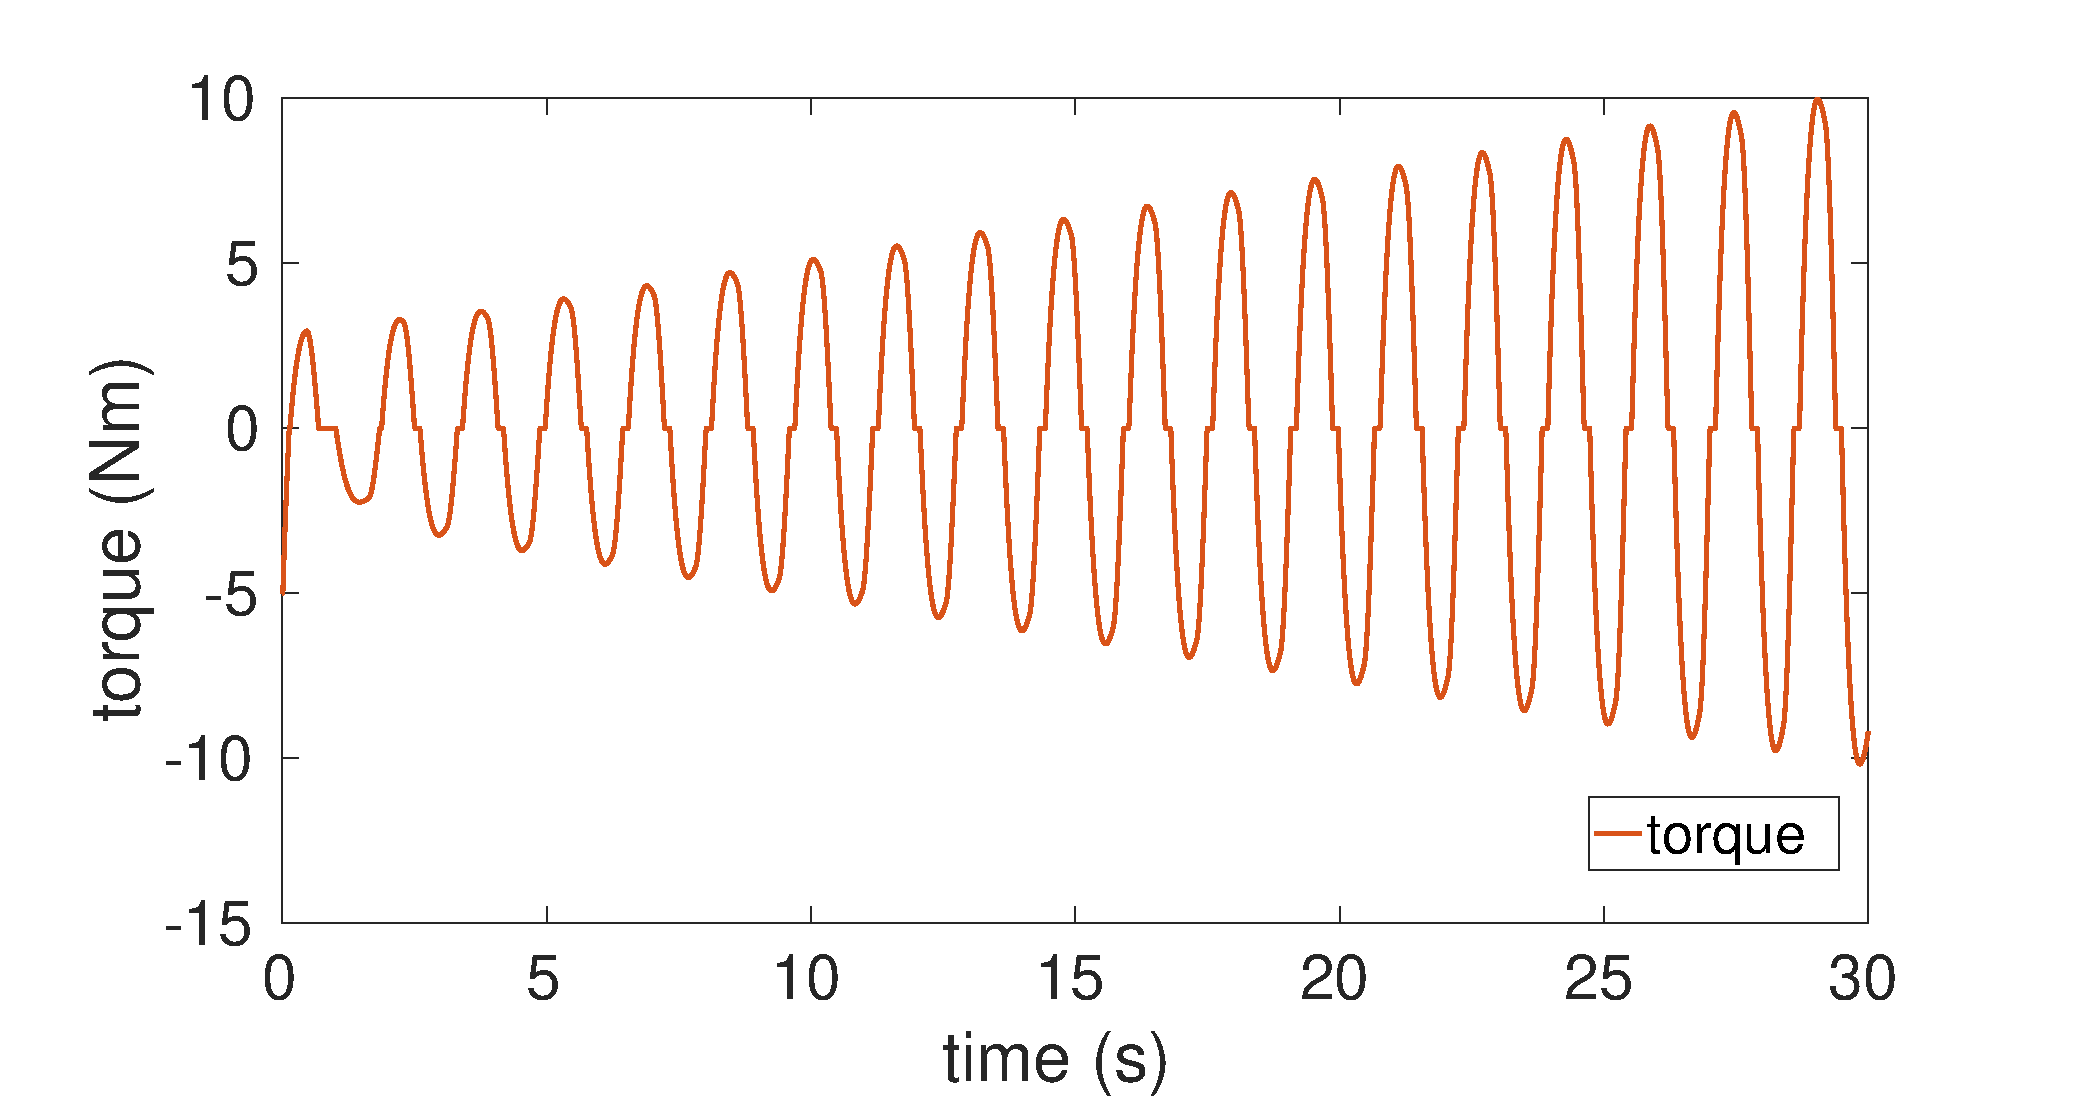
\includegraphics[scale=0.30]{figures/2-1-change-in-torque.eps}}
\subfigure[Joint position and average joint position]{\label{fig:a}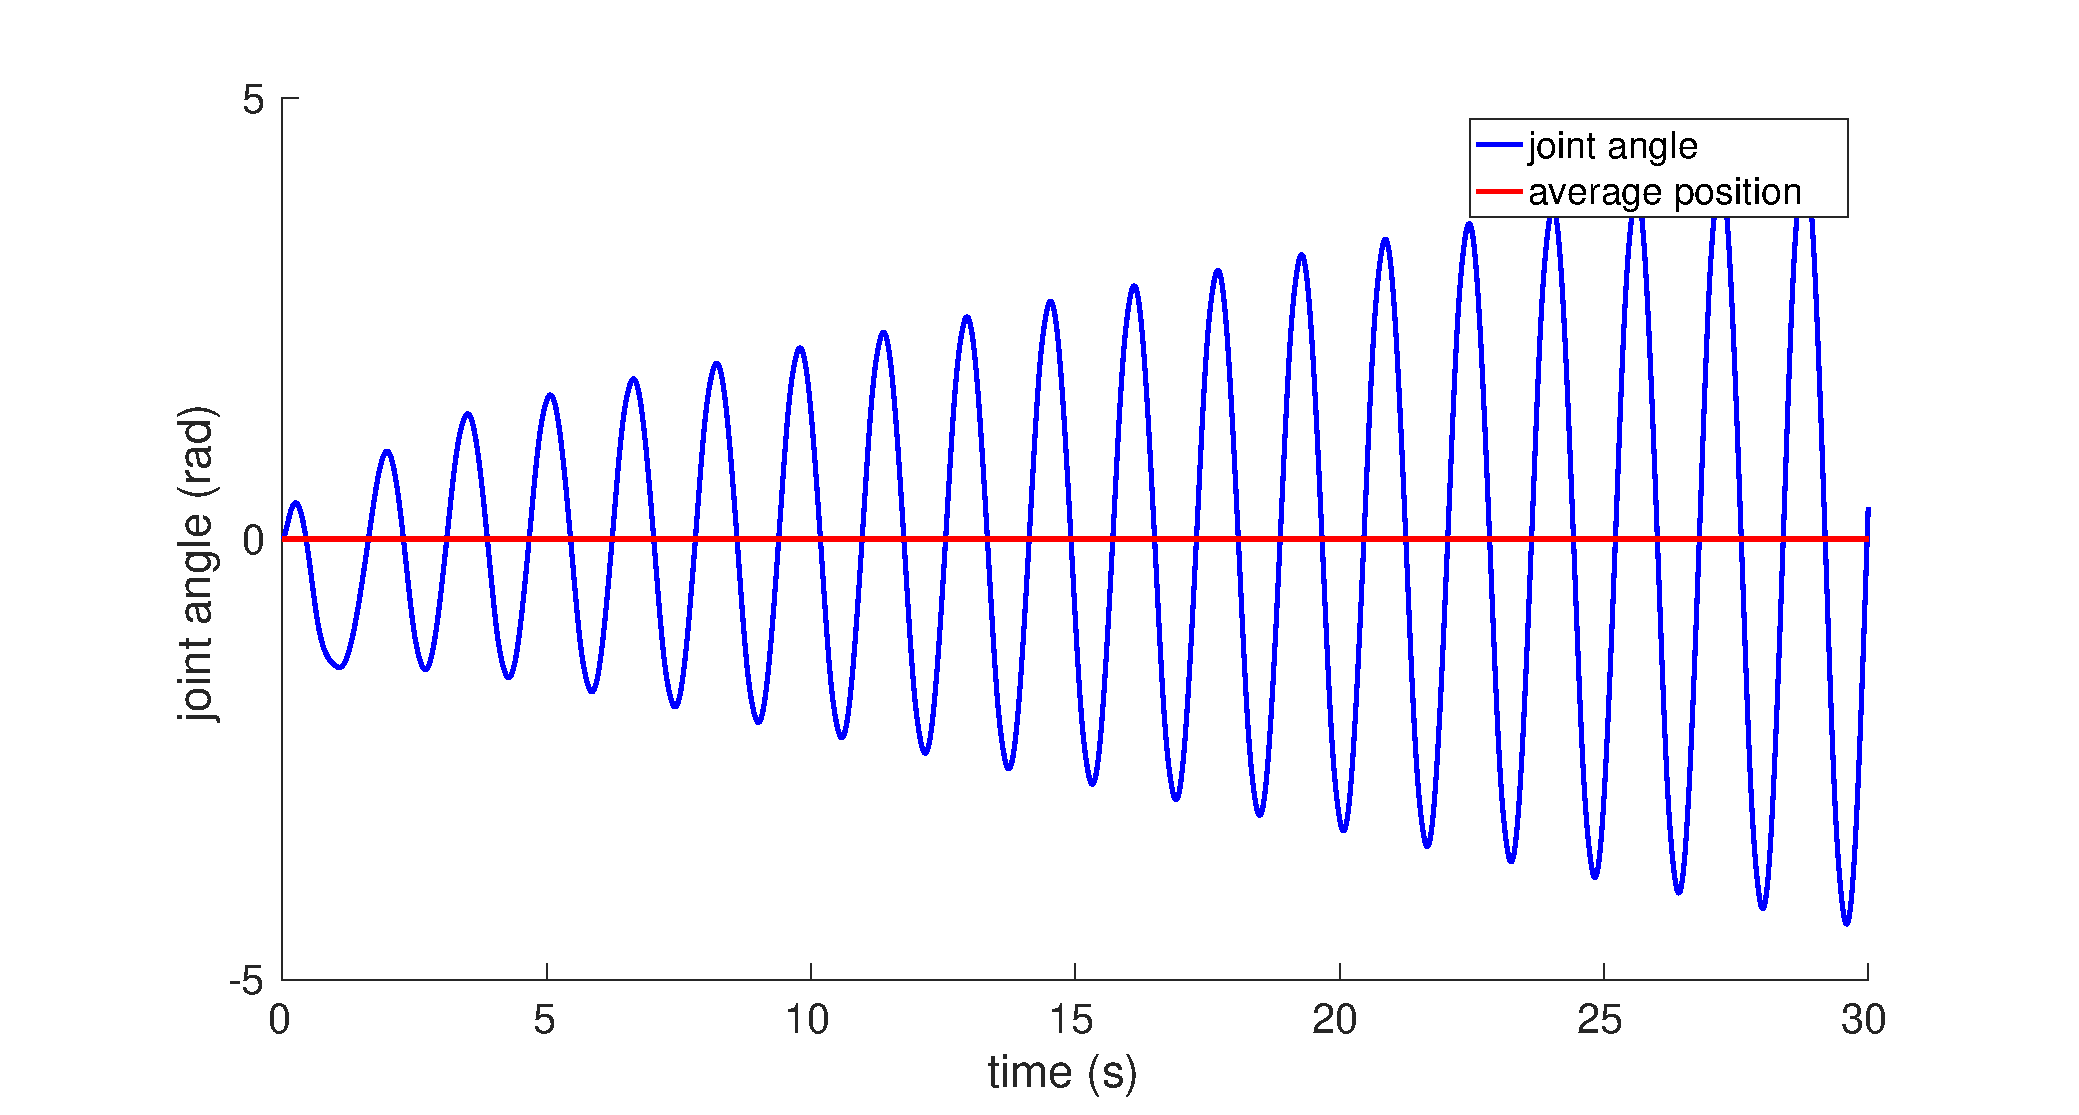
\includegraphics[scale=0.30]{figures/2-2-change-in-angle.eps}}
\subfigure[Tonic input to the oscillator]{\label{fig:b}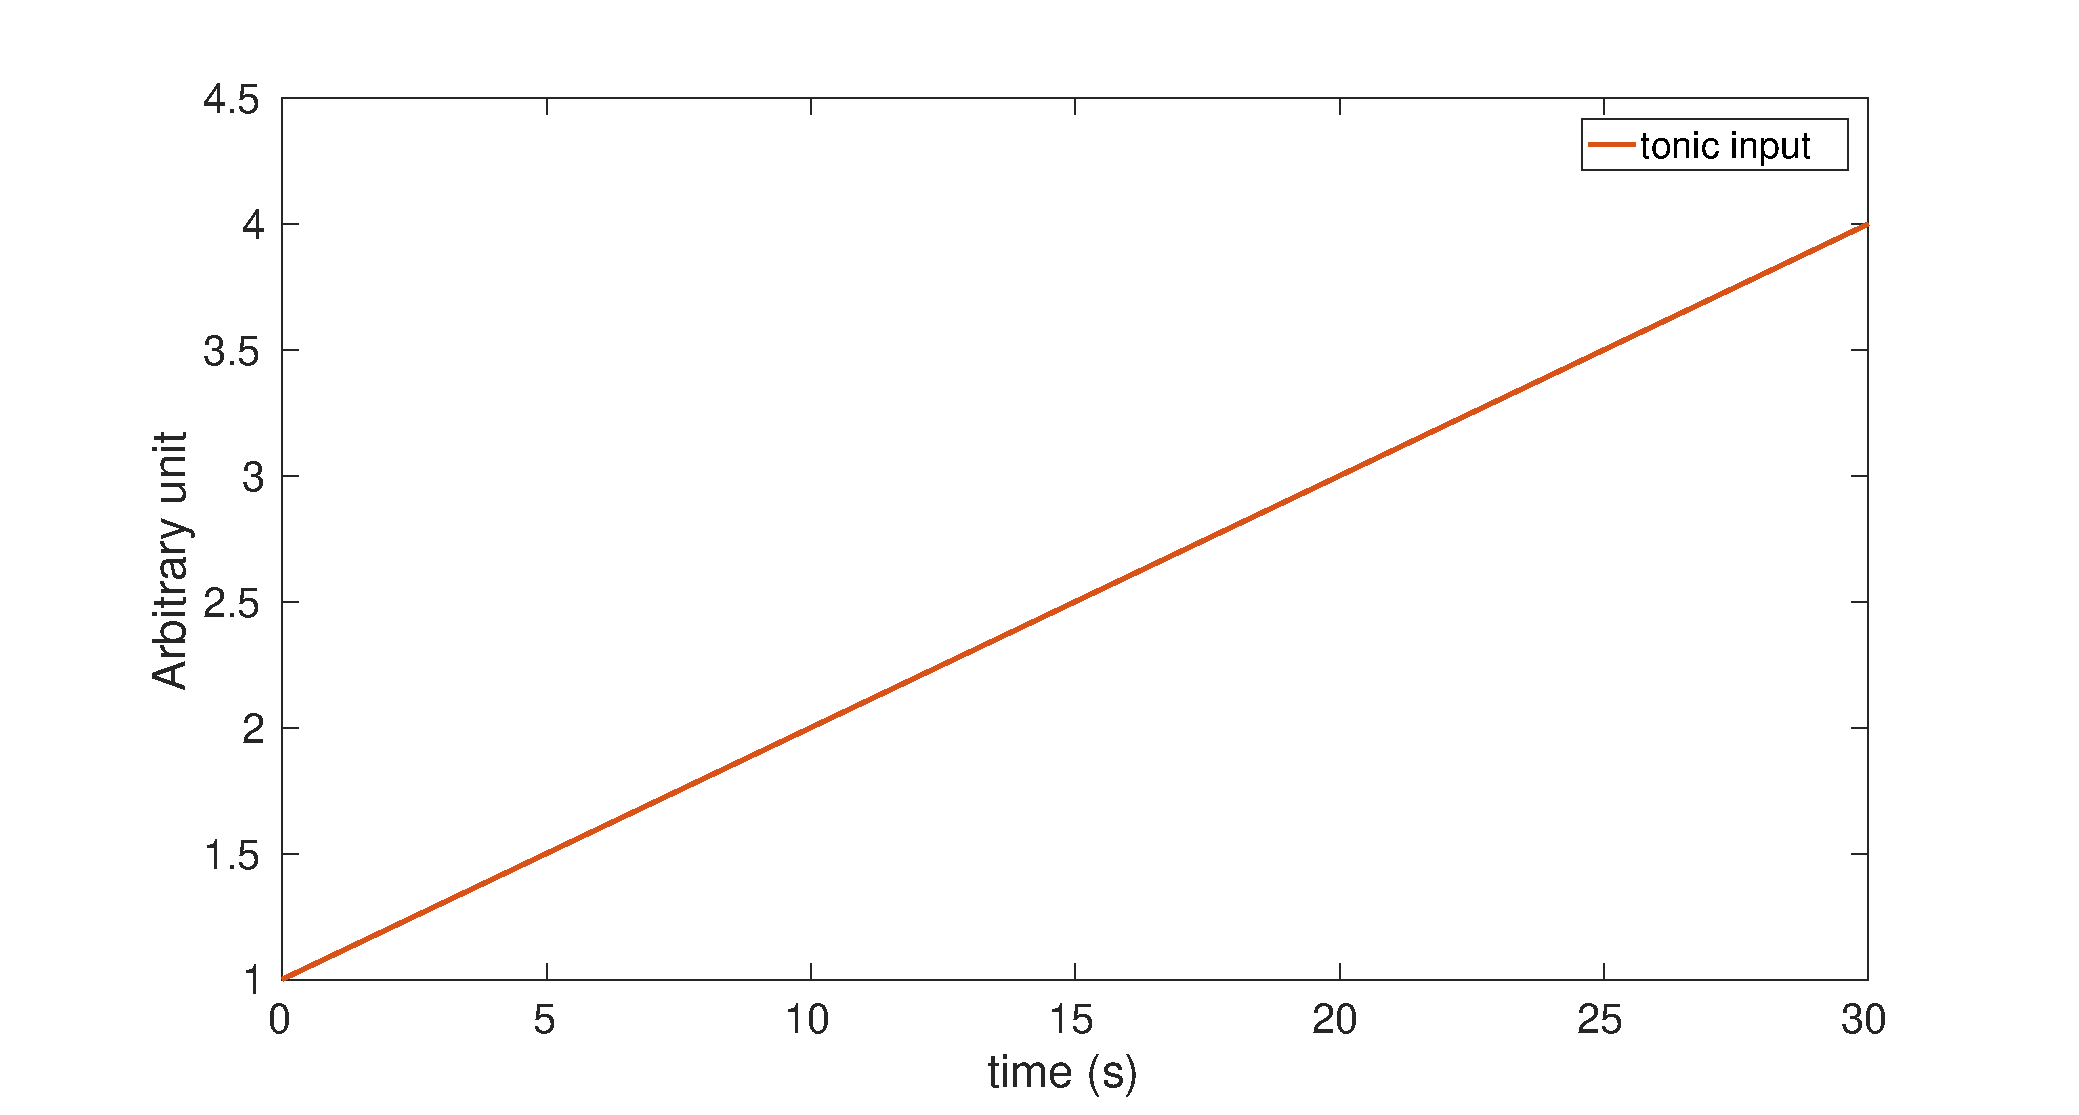
\includegraphics[scale=0.30]{figures/2-3-change-in-ut.eps}}
\caption{Changing the amplitude of oscillations}
\label{fig:change-amp}
\end{figure}

\subsection{Controlling the frequency of the joint angle oscillations}
By varying the time constants of the oscillator the frequency of the torque and joint angle oscillations can be varied. In figure \ref{fig:change-freq}, the time constant $t_1$ was set to 0.3 for the first 20 seconds, 0.6 for the next 20 seconds and to 0.9 for the last 20 seconds. The constant $t_2$ was set as $t_2 = 2.5 \times t_1$ as in \cite{ronsse2009computational}. As expected the frequency of both the torque and the joint angle oscillations decreases. However for the joint angles, the amplitude also increases as the frequency decreases. Throughout the 60 seconds, the tonic input $u_t$ was set to 1. Note that for both the 2 changes (at $t=20s$ and $t=40s$), the transitions were smooth.

\begin{figure}[htbp]
\centering     %%% not \center
\subfigure[Torque output of the oscillator]{\label{fig:b}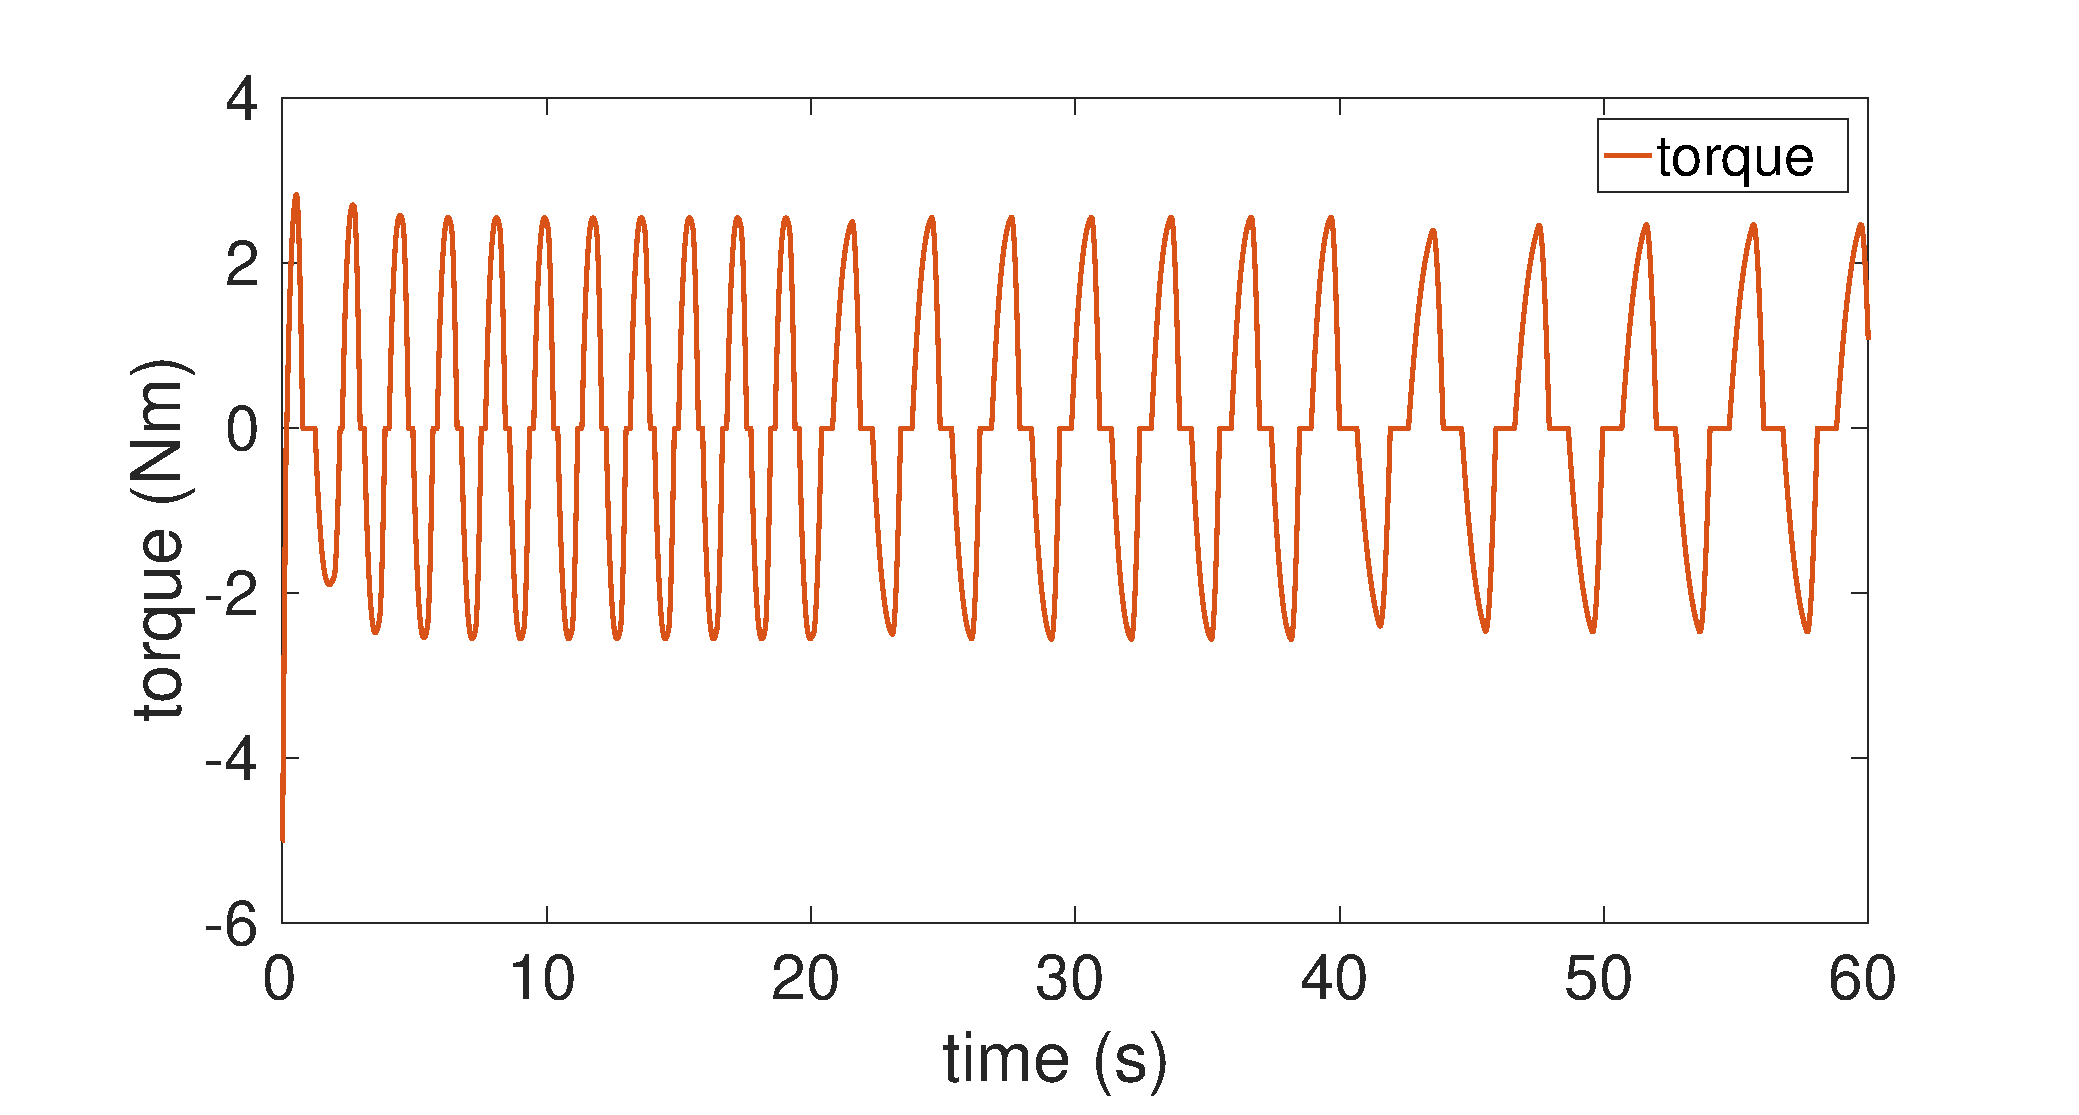
\includegraphics[scale=0.33]{figures/3-1-changing-freq-torque.eps}}
\subfigure[Joint position and average joint position]{\label{fig:a}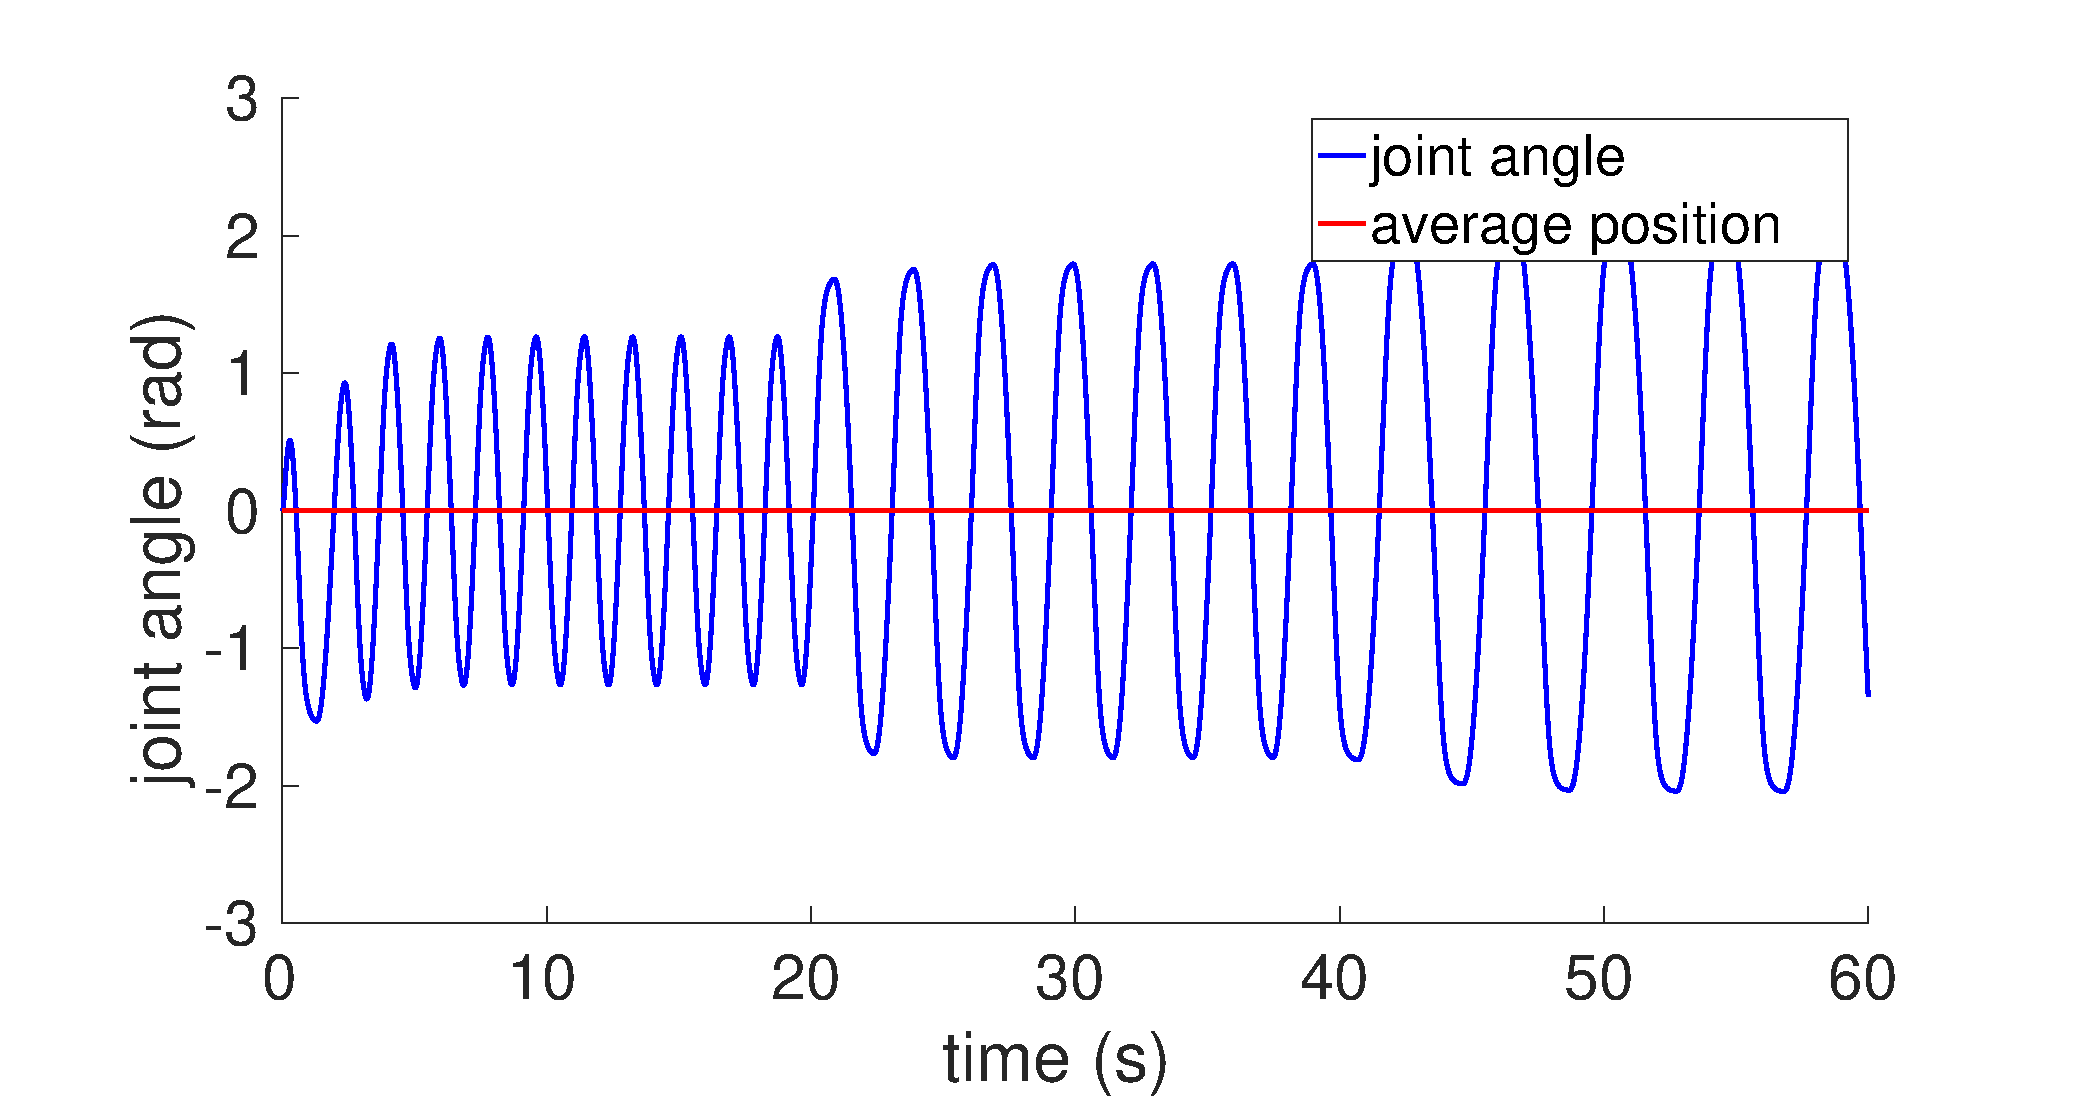
\includegraphics[scale=0.33]{figures/3-2-changing-freq-pos.eps}}
\caption{Changing the frequency of oscillation}
\label{fig:change-freq}
\end{figure}

\section{Conclusion}

\cite{ronsse2009computational, williamson1998neural, matsuoka1987mechanisms, matsuoka1985sustained}

%%%%%%%%%%%%%%%%%%%%%%%%%%%%%%%%%%%%%%
% hier werden - zum Ende des Textes - die bibliographischen Referenzen
% eingebunden
%
% Insbesondere stehen die eigentlichen Informationen in der Datei
% ``bib.bib''
%
\bibliographystyle{plain}
\bibliography{SA}
\end{document}


